\documentclass[11pt,a4paper]{article}
\usepackage[margin=25mm]{geometry}
\usepackage[T1]{fontenc}
\usepackage{lmodern,microtype,amsmath,amssymb,booktabs,tabularx,longtable,graphicx,enumitem}
\usepackage[hidelinks]{hyperref}
\newcolumntype{Y}{>{\raggedright\arraybackslash}X}
\setlist{nosep}\emergencystretch=1.5em
\renewcommand{\thesection}{S\arabic{section}}
\renewcommand{\thetable}{S\arabic{table}}
\renewcommand{\thefigure}{S\arabic{figure}}
\title{Online Resource 1: Supplementary information\\Operational limits of reference renewal for retained quantum-service results}
\author{\begin{tabular}{c}
\normalsize \href{https://orcid.org/0009-0003-5312-2634}{Roberto Fernández-Barrios}, \href{https://orcid.org/0000-0002-3068-6248}{Iker Pastor-López},\\
\normalsize \href{https://orcid.org/0009-0003-9080-6242}{Amaia Pikatza-Huerga}, \href{https://orcid.org/0000-0003-3594-9534}{Pablo García Bringas}\\[5pt]
\small Faculty of Engineering, University of Deusto,\\
\small Avda. de las Universidades 24, 48007 Bilbao, Spain\\[4pt]
\small Corresponding author: Roberto Fernández-Barrios\\
\small \href{mailto:roberto.fernandez.b@deusto.es}{roberto.fernandez.b@deusto.es}
\end{tabular}}
{}\date{}
\begin{document}\maketitle
\noindent This supplement accompanies the manuscript prepared for \emph{Quantum Information Processing}. Campaign B is the principal evaluation; Campaign A retains its own locally fixed protocol and is an antecedent relative to B. Sections S2.3, S5 and S6 identify earlier retrospective clarifications; S8 identifies the retrospective analyses introduced in v5 and the descriptive context comparison added in v5.1. None changes an endpoint, threshold, scientific population or historical verdict. The canonical result is eight successes in ten usable windows, exact one-sided $p=0.0546875$, H1-B not established.

\section{Relationship to the authors' other work}
The closest predecessor is \emph{Observational Indistinguishability and Integrity Blind Regions in Hybrid Quantum-Classical Workflows} (Fernández-Barrios, Pastor-López, Pikatza-Huerga and García Bringas, \cite{fernandez2026observational}). It develops claim-relative evidence views, structural blind regions, reference sufficiency, offline policy analyses and an ideal-statevector/finite-shot-emulation branch. Its empirical scope explicitly excludes physical quantum processing unit (QPU), provider and deployed-service assurance. This study inherits the evidence/reference perspective, kernel lineage and calibration discipline. It contributes neither a new evidence lattice nor a new general integrity theorem. Its additional object is a physically executed reference-renewal sequence and a prespecified service endpoint, with provider-dependent binding and explicit costs. The two studies do not supply independent replications of the same hypothesis.

Other work by the authors sets related boundaries. \emph{Candidate Comparability Before Promotion: Conditional Validation in Adaptive Network Intrusion Detection} (Fernández-Barrios, Pastor-López, Pikatza-Huerga and García Bringas, \cite{fernandez2026candidate}) studies how challenger construction and evidence alter promotion conclusions and policy rankings. \emph{Sharp Target-Domain Certificates for Quantum-Kernel Advantage under Distribution Shift} (Fernández-Barrios, Pastor-López, González-Santocildes and García Bringas, \cite{fernandez2026certificates}) derives identified intervals for predictive advantage over a fixed classical family under missing target labels. \emph{The Price of Missing Labels in Certification with Unknown Readout} (unpublished submitted manuscript) studies minimax label and measurement acquisition under a fixed statistical contract. The revised collider-classifier auditing manuscript, \emph{Information and reference requirements for auditing collider classifiers} (Fernández-Barrios, Pastor-López, González-Santocildes and García Bringas, \cite{fernandez2026collider}), explains reference-dependent claims and descriptive auditing evidence, with withdrawn physical-coverage conclusions explicitly excluded. This study does not claim any of those results again, measure predictive quantum advantage, prove an acquisition optimum or repair that manuscript's withdrawn conclusions. Their shared principle of specifying evidence before asserting a claim is not presented as a new method here.

The main-text description of Beisel et al. is limited to the publisher abstract; its full text was not inspected. This scope note does not imply a full-text comparison.

The bibliography identifies the public preprint versions, not journal acceptance. No journal DOI is asserted for these preprints. The unpublished certification-cost manuscript is mentioned only to delimit the contribution; no public identifier has been established for it.

\section{Campaign A: original result and developmental role}
\subsection{Original population and inference}
A was prespecified under \texttt{paper25-prereg-v1}, with three documented amendments. It stopped at its maximum of 12 candidate epochs. Nine were accepted: C01/W01 bootstrap; C03--C07/W02--W06 usable transitions; and C10--C12/W07--W09 accepted with execution failures and non-usable. C02, C08 and C09 were incomplete. Bootstrap is not a transition; hence the nine accepted windows are not nine usable transitions.

Its primary estimand was the mean window-level paired difference in unsafe service continuation, P5 minus P2. Five usable windows yielded 30 paired probes. Both policies served zero oracle-incorrect primary results (0/30 each); each window's descriptive difference was zero. P2's 30 services were assurance-invalid under the context criterion, while P5's 30 were valid. That difference concerns eligibility under the policy definitions and is not prevention of observed errors.

A required at least eight usable windows. With five, the longitudinal minimum was unmet (kill criterion KC2), the frozen primary inference was not computed, and H1-A was not established. No reduced-sample test or confidence interval is supplied here. The original closure also records the absence of stale-rule degradation in the usable population and the resulting claim restrictions. B's endpoint is not retroactively applied to A.

\subsection{Operational observations that informed B}
A's 527 attempt records cover 521 logical units with at least one record and 524 provider-accepted submissions. The local acquisition produced 493 sealed results and 31 local timeouts under its 3,600 s rule. The historical closure reports that all 31 later reached provider DONE; they remain audit-only, without scientific envelopes or promotion into the primary population. This statement relies on the preserved historical reconciliation, not a fresh provider query. The closure records 1,572 conservative QPU seconds and 984 provider-reported seconds. These are resource accounting values, not measured end-to-end latency, energy or invoice cost.

The three accepted non-usable transitions lost primary probes: C10 retained 4/6, C11 2/6 and C12 4/6. C11's reference had only 33/39 calibrations. The three incomplete candidates terminated when their workload-context digest changed during acquisition. Their local admission-to-completion intervals were 5,022.302 s (C02), 21,390.668 s (C08) and 33,009.957 s (C09). These are neither physical context lifetimes nor direct provider queue measurements.

B's design report explicitly links these observations to a provider-aware terminal-state policy, an admission gate using active status and queue depth, historical execution binding, an irrevocable context-expiry/window-time limit, a target of ten \emph{usable} transitions and separate fallback reporting. A's operational metadata was used for gate design; the historical record states that scientific outcomes were not used to choose the gate threshold. The absence of observed unsafe service in A was a separate motivation for changing the primary question to timed recovery. The workload, oracle and calibrated score rule were retained. A also had controlled optimization-level stress probes that B removed. Protocol and period differences preclude causal attribution of different completion counts or latency summaries to any individual design change.

\subsection{Retrospective reference-field reconciliation}
The original A closure reports six successful recalibration flags across accepted transitions. The later operational inspection found seven complete transition references. These count different objects. The code records the flag on a sealed P5 probe with suffix 01; C12 completed 39/39 calibration units but its probe 01 failed and generated no such flag. C11 had 33/39 calibrations and two scientific P5 fallback records under A's original rules. Those records must not be recast as valid retained-result recovery under B's stricter complete-reference rule.

\begin{table}[htbp]\centering\small
\begin{tabular}{lrrrr}\toprule
A candidate & Calibrations & Complete & Recalibration flags & Scientific primary P5\\\midrule
C03--C07 & 39 each & Yes & 1 each & 6 each\\
C10 & 39 & Yes & 1 & 4\\
C11 & 33 & No & 0 & 2\\
C12 & 39 & Yes & 0 & 4\\\bottomrule
\end{tabular}
\caption{Retrospective reconciliation, not a replacement of A's endpoint. The flag count and complete-reference count use different units.}\label{tab:a_reference}
\end{table}
The archived \texttt{A\_reference\_semantics.csv} and \texttt{A\_timeout\_attempts.csv} retain the finer detail. No missing outcome is imputed, no late result is rescued and no B binding classification is assigned to A.

\section{Campaign B contract, population and evidence units}
\subsection{Normative contract and amendments}
The original B freeze tag is \texttt{paper25b-prereg-v1}, commit \texttt{fccb712}. Amendments 1--3 resolve frozen-digest scope, the pre-provider request boundary and launch-record provenance, respectively; their effective commits are \texttt{3a23b2f}, \texttt{88f65e9} and \texttt{34663b6}. They retain the hypotheses, endpoint, thresholds and population rules. Amendment 1 was authorized on 7 October before acquisition; amendment 2 on 10 October after C01's halt, with zero provider jobs or physical outcomes; amendment 3 on 12 October after C01--C03, with 88 accepted jobs and one usable transition. C04 had not opened. It preserves the earlier evidence and documents the provenance exception for the legacy launch record. All three are disclosed as amendments, not hidden behind a claim of an unchanged executable throughout acquisition. The preregistration source retains an obsolete pre-freeze header; the annotated tag and freeze record make those exact bytes normative. It is not an unfrozen protocol merely because the historical header was preserved.

Acquisition closed at C14 on 25 October 2026 (commit \texttt{a11cf9c}); final analysis is \texttt{4be9c01}; documentary review v1.1 is \texttt{2c1fd72}. The historical closure dossier records the full identifiers and amendment chain. Online Resource 2 supplies the relevant protocol documents and source identities as a derivative export. Its v1.1 correction narrows the independence wording for clustered binding failures; no numerical result changes. This article uses that corrected interpretation.

The target was ten usable transitions, subject to at most 16 candidate epochs, 810 ledger-budgeted jobs, 2,430 conservative QPU seconds, quota guards, fatal criteria, 90 calendar days and 30 days without a gate-open opportunity. The campaign stopped on usable count, not on the accumulating success count. The six service probes, 39 reference jobs and two verification jobs give 47 jobs per complete transition; bootstrap has 41. The 1,800 s deadline was retained from the service contract; the design report describes it as providing margin relative to A's observed recovery times under low queue conditions, not as an externally validated industrial service-level agreement. The five-retained/one-fallback restriction is the author-specified safeguard against an all-classical success. The null of 0.5 and ten-window, nine-success rule are prospectively chosen evaluation criteria; the design does not derive 0.5 from a deployment requirement or a competing policy. They are not population reliability targets of 0.8 or 0.9. Unit assignment and replay order are randomized within the fixed sequential stage design by a committed seed. They do not randomize P2/P4/P5 physical treatment arms.

\subsection{Selection and the complete candidate flow}
\begin{table}[htbp]\centering\small
\begin{tabular}{llrrrrr}\toprule
Candidate & Role & Jobs$^a$ & Bound & Unbound & Reference & Ledger\\\midrule
C01 & Bootstrap & 0 & 0 & 0 & 0/39 & 28\\
C02 & Bootstrap & 41 & 41 & 0 & 39/39 & 41\\
C03 & Usable & 47 & 47 & 0 & 39/39 & 47\\
C04 & Usable & 47 & 47 & 0 & 39/39 & 47\\
C05 & Incomplete & 43 & 36 & 7 & 30/39 & 43\\
C06 & Usable & 47 & 47 & 0 & 39/39 & 47\\
C07 & Usable & 47 & 47 & 0 & 39/39 & 47\\
C08 & Usable & 47 & 47 & 0 & 39/39 & 47\\
C09 & Incomplete & 29 & 28 & 0 & 22/39 & 29\\
C10 & Usable & 47 & 47 & 0 & 39/39 & 47\\
C11 & Usable & 47 & 47 & 0 & 39/39 & 47\\
C12 & Usable & 47 & 47 & 0 & 39/39 & 47\\
C13 & Usable & 47 & 47 & 0 & 39/39 & 47\\
C14 & Usable & 47 & 47 & 0 & 39/39 & 47\\
\bottomrule
\end{tabular}
{}
\caption{All B candidate epochs, including incomplete attempts. $^a$Provider-accepted jobs: includes one subsequently cancelled job and does not assert physical execution for every acceptance. Bound/unbound count only units reaching the corresponding evidence classification. Ledger is conservative budget accounting.}\label{tab:bflow}
\end{table}
The gate conditions on backend active/operational status, executable support, queue depth at most five, a genuinely new workload-context digest and strictly later calibration timestamp. It requires two qualifying snapshots at least 600 s apart and another check immediately before opening. These are observations at admission; they do not reserve capacity for all subsequent work. No queue-depth throttling is applied after opening.

Usability additionally requires six bound held probes, 39 bound calibration units, an integrity-verified complete reference and re-evaluation before scientific expiry. The gate and usability are distinct selection stages. Usability is decided without inspecting the final recovery verdict, but completion and binding can still be associated with the latency endpoint. The nominal target probability concerns gate-admitted genuine transitions; the test actually observes only the usable subset. Extrapolation to all admissions requires additional assumptions not established by this study. Table~\ref{tab:bflow} exposes the exclusions without changing the frozen denominator of ten.

C01 halted before any provider-accepted job. Its 28 pre-boundary submission failures consumed conservative ledger entries; they were not 28 QPU executions. C05 expired with only 30 bound calibrations and seven J3 failures. C09 expired during calibration; its outstanding job was cancelled by the runner under the context-expiry rule. Each had six bound held service probes, but neither obtained a complete reference before expiry. This is a retrospective flow clarification, not an alternative estimand or test over twelve transitions. Scientific expiry is irrevocable. No post-window result can restore usability or repair a reference; no late result was promoted.

\subsection{Units and accounting}
There are 613 attempt records: 575 BOUND\_SEALED, 7 UNBOUND\_AUDIT\_ONLY, 1 CANCELLED\_BY\_RUNNER, 28 SUBMIT\_FAILED and 2 NOT\_SUBMITTED. They cover 612 logical units with some record, not every planned unit in aborted windows. Provider acceptance totals 583 (582 DONE and one CANCELLED). The ledger totals 611, comprising 583 acceptances plus the 28 early failures. The provider-reported charge is 1,164 s; conservative accounting is $611\times3=1,833$ s. The single recorded acquisition retry was C01 unit \texttt{B01-calibration-27}. Attempts 1 and 2 both ended SUBMIT\_FAILED before provider acceptance; the second is explicitly linked to the first. This one logical unit accounts for the 613-versus-612 difference. Neither attempt executed physically or produced held evidence. There are zero service-probe reruns after HOLD.

For C09 unit \texttt{B09-calibration-11}, the saved cancellation record gives provider status QUEUED at the runner's request, at 09:08:37.545415 UTC on 19 October. Scientific termination was recorded at 09:08:38.378442, and CANCELLED was observed at 09:09:08.872742. This is consistent with the rule permitting cancellation of queued jobs on context expiry, without cancelling a job observed running. A separate runner-loss incident on 15 October occurred before any C09 window opened or unit was submitted; it must not be placed inside the later acquired window. This retrospective narrative clarification changes no classification or endpoint.

One job carries the six circuits used to form the kernel, each with shot setting 128. Circuits, shots, attempts, logical units, policy records, probes and windows are different units. The 60 primary probes share ten references. The 82 records per policy across accepted windows comprise 60 primary and 22 verification records; replaying three policies does not triple the number of physical experiments.

The stored \texttt{windows\_lost\_to\_unbound\_units}=0 counts accepted windows demoted to non-usable by required-phase binding failures. It excludes incomplete C05. Consequently it means no \emph{accepted} window was demoted by binding, not that no candidate was affected. Similarly, local \texttt{done}=575 in B counts sealed outcomes, while provider DONE=582 includes the seven audit-only outcomes. A's local \texttt{done}=493 has its own timeout-based semantics. The accompanying data dictionary explains why these are not interchangeable completion rates.

\section{Primary and descriptive secondary results}
\subsection{Frozen primary inference}
The nominal model is ten independent Bernoulli windows with common probability $\pi_B$, tested against $H_0:\pi_B\leq0.5$ with a one-sided exact binomial test at $\alpha=0.05$. Rejection requires at least nine successes. The observed eight give $p=7/128=0.0546875$; the two-sided 95\% Clopper--Pearson interval is $[0.4439045377,0.9747892737]$ and the one-sided 95\% lower bound is 0.4930986989. H1-B is not established. Removing either failed window leaves 8/9 successes; removing any successful window leaves 7/9. These are the required descriptive leave-one-window-out counts, not alternative tests.

Temporal dependence and heterogeneity remain possible. Five usable windows, W07--W11, opened within four hours on 25 October. A context digest change does not generate independence; exactness of the binomial calculation is conditional on its statistical model. Integrity controls do not establish that model. No dependence-adjusted estimate, intracluster correlation, reduced-$n$ test, alternative cutoff or secondary promotion is introduced.

\subsection{Policies, sources and endpoint distinctions}
\begin{table}[htbp]\centering\small
\begin{tabular}{llrrrrr}\toprule
Policy & Phase & Records & Served & Correct$^a$ & Valid$^a$ & Timed success\\\midrule
P2 & Primary & 60 & 57 & 57 & 0 & --\\
P4 & Primary & 60 & 0 & 0 & 0 & --\\
P5 & Primary & 60 & 60 & 60 & 60 & 48\\
P2 & Verification & 22 & 21 & 21 & 21 & --\\
P4 & Verification & 22 & 21 & 21 & 21 & --\\
P5 & Verification & 22 & 22 & 22 & 22 & --\\\bottomrule
\end{tabular}
\caption{Phase-specific policy records. $^a$Among served outputs. A dash means that the relevant recovery clock was not measured, not zero success. Verification includes bootstrap and uses the window's own completed reference, so its served outputs can be support-valid under P2/P4.}\label{tab:policy}
\end{table}
In policy replay, P2 uses the most recent prior accepted, complete, bound and integrity-verified reference, even though its support no longer matches the new context. It is calibration-invalid if no such reference exists. P4 checks support and withholds. P5 physically renews the reference and re-evaluates the same held result. The 57 primary outputs that the P2 replay would serve were numerically correct but assurance-invalid; the three other probes were rejected by its calibrated rule. All 60 held primary physical results were oracle-correct, including the four replaced by P5 and the three rejected in the P2 replay. This follows from the physical-result oracle fields, not merely from the correctness of served fallbacks. No nominal false-rejection guarantee is inferred from these counts. Hence the experiment observes no differential error prevention.

P5 served 56 retained primary outputs and four classical fallbacks. Primary fallbacks occurred in W02, W03, W06 and W07; a fifth fallback occurred separately in verification at W04. Fallback uses the exact classical matrix already accessible to the workload, and is correct by construction under that oracle. It is a different service source. The frozen primary endpoint permits at most one fallback per window only after bound held evidence, a complete reference and a rejected re-evaluation. It cannot rescue missing or unbound evidence.

The retained-only endpoint requires all six probes to satisfy the timely-valid-service rule \emph{and} all six sources to be retained physical results. It succeeded in W05 and W08--W11: 5/10. It is not the 56/60 retained fraction. W04 retained all six but failed the deadline; W02, W06 and W07 met the primary endpoint with one fallback each. These distinctions expose how much of the observed primary success depends on classical replacement.

\begin{table}[htbp]\centering\small
\begin{tabular}{lrr}\toprule
Endpoint / scope & Count & Nominal Wilson 95\%\\\midrule
P2 primary assurance-invalid & 57/60 & [0.8630, 0.9829]\\
P5 assurance-invalid, both phases & 0/82 & [0.0000, 0.0448]\\
Retained outputs, primary & 56/60 & [0.8407, 0.9738]\\
Fallback outputs, primary & 4/60 & [0.0262, 0.1593]\\
P2: Incorrect among served & 0/78 & [0.0000, 0.0469]\\
P4: Incorrect among served & 0/21 & [0.0000, 0.1546]\\
P5: Incorrect among served & 0/82 & [0.0000, 0.0448]\\
P2: Mixed-clock availability & 21/82 & [0.1740, 0.3600]\\
P4: Mixed-clock availability & 21/82 & [0.1740, 0.3600]\\
P5: Mixed-clock availability & 70/82 & [0.7614, 0.9143]\\
P2: Verification correct services & 21/22 & [0.7820, 0.9919]\\
P4: Verification correct services & 21/22 & [0.7820, 0.9919]\\
P5: Verification correct services & 22/22 & [0.8513, 1.0000]\\
Binding failure, DONE units & 7/582 & [0.0058, 0.0246]\\
Retained-only window success & 5/10 & [0.2366, 0.7634]\\
\bottomrule
\end{tabular}
{}
\caption{Canonical descriptive rates and nominal intervals. The last two intervals were completed in the historical documentary closure. None is adjusted for within-window or temporal dependence; none establishes a population reliability guarantee or supersedes the primary result.}\label{tab:rates}
\end{table}

The aggregate availability field applies the 1,800 s clause only to records carrying T0--T3; elsewhere it defaults to true. Thus 70/82 for P5 is 48 timed primary successes plus 22 verification services, while P2 and P4 each contribute 21 untimed verification services. Table~\ref{tab:policy}, rather than that mixed aggregate, identifies what each policy actually did. P2/P4 are replays on shared physical evidence and have no independently measured competing latency.

\subsection{Coverage of all prespecified descriptive endpoints}
The secondary outputs remain available in \texttt{data/secondary\_endpoints.json}; Table~\ref{tab:rates} retains every reported rate and interval. The remaining quantities are: recovery latency across 60 primary records (median 666.0264885 s, range 565.561698--26885.649444 s); reference-ready latency (ten distinct shared intervals, range 565.495767--24719.410329 s); provider queue wait over 582 DONE binding-classified units (median 1.2706435 s, maximum 19532.816135 s); reference cost (390 calibrations in usable transitions, plus 39 in bootstrap); incomplete and missing units (S3); and queue/resource exposure (S3 and S5).

The frozen reference-latency summary repeats each window's T1--T2 value for its six probes, yielding 60 records and median 634.9956285 s. There are only ten acquired references, not 60 independent recalibrations. The table of usable windows and supplied machine-readable rows preserve the distinct values.

Recorded queue-exposure counters are 5,461 polls, 1,251 gate-open polls, 2,983 gated-candidate polls, 14 candidate rollovers and 14 openings. They are counters in saved state, not a continuous-time availability measure or independent episodes. Maximum sampled queue depths in C04 and C06 were 64 and 1,912 despite depth one at opening. No threshold is fitted to these observed maxima. The three observation times for admission are retained in the retrospective timing table; they need not have identical queue depths.

The record field \texttt{trusted\_invariants\_held} is populated from \texttt{outcome.binding\_valid} in the frozen runner, not from an independent global invariant verifier. The runner verifies the HMAC it has just created; the flag defaults to true, including for some failed/unbound attempts. It must therefore be combined with the distinct execution and J1--J4 predicates and remains a local self-verification premise, not independent evidence of physical authenticity. Local ``served'' records are the service outcomes measured here; external client delivery was not timed. The primary safety gate found zero violations. KC-B1 through KC-B9 were not triggered in the observed analysis. This includes zero incorrect P5 services in either accepted phase; it does not establish complete future enforcement (S7.3).

\section{Retrospective timing clarification}
T0 is each probe's HOLD after sealing; T1 is the first calibration submission; T2 is reference readiness; T3 is service or terminal rejection. T3--T0 includes later primary-probe acquisition, waiting, calibration, orchestration and re-evaluation after that HOLD. It excludes all acquisition before that probe's HOLD and any preceding user-request interval. Each probe has a different T0 even though the reference is shared. The 1,800 s endpoint is not implemented as a hard late-output cutoff.

\begin{figure}[htbp]\centering
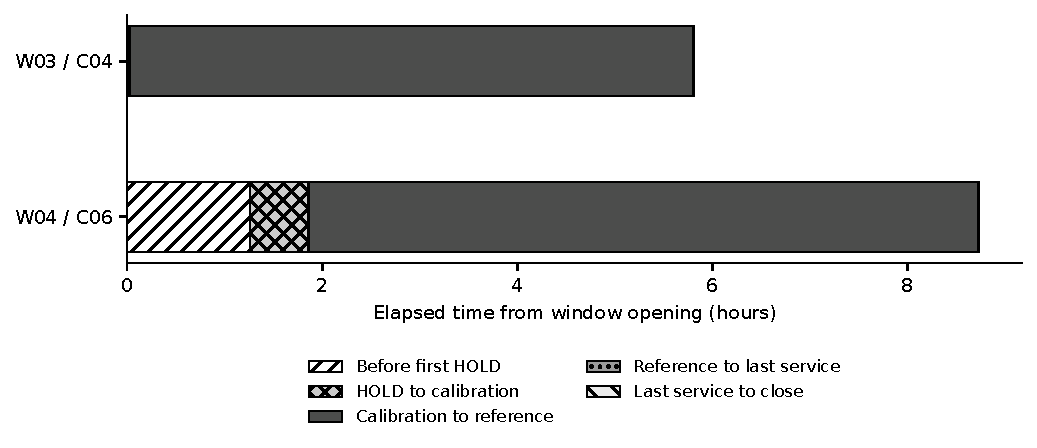
\includegraphics[width=\linewidth]{figures/FigS1.pdf}
\caption{Retrospective local-clock partitions of the two failed windows, each measured once. Very short post-reference segments are present but visually small. Window duration is not the same clock as any individual HOLD-to-service endpoint.}\label{fig:clock}
\end{figure}
\begin{table}[htbp]\centering\small
\begin{tabular}{lrr}\toprule
Observed local interval (s) & C04 & C06\\\midrule
Opening to first HOLD & 17.027 & 4528.160\\
First HOLD to calibration start & 77.764 & 2166.235\\
Calibration start to reference ready & 20789.767 & 24719.410\\
Reference ready to last service & 0.051 & 0.047\\
Last service to window close & 41.921 & 32.072\\
Complete window & 20926.530 & 31445.924\\\midrule
Provider calibration queue sum & 19606.429 & 23570.316\\
Provider calibration execution sum & 878.703 & 713.662\\
Reference interval minus both sums & 304.635 & 435.432\\\bottomrule
\end{tabular}
\caption{Rounded display of the retrospective partitions; full precision is in \texttt{B\_clock\_partitions.csv}. Provider intervals use a different clock source and do not partition the whole service clock.}\label{tab:clock}
\end{table}
The 39 provider calibration intervals were checked as non-overlapping and nested in each local reference interval. This allows their arithmetic comparison but does not identify the residual as exclusively local overhead: communication, observation, local work and clock semantics remain combined. The sum of queue durations is an observed association, not an estimated causal delay contribution. Removing it would not reconstruct the system, scheduling or calibration context under a different queue.

C06's first probe waited a provider-reported 4,473.832 s before its HOLD. After that HOLD, 2,166.235 s elapsed before the first calibration submission. The earliest-held probe therefore missed the 1,800 s endpoint before any calibration job was submitted; sequential acquisition of the remaining probes is a separate deadline risk. Pre-HOLD acquisition matters to full-window accounting, while later probe acquisition is included in that first probe's recovery clock. The maximum per-probe recovery duration and the last service have different starting/ending boundaries. Figure~\ref{fig:clock} uses the explicitly recorded boundaries instead of subtracting unrelated extrema.

C09's outstanding job took 22,869.500 s from recorded acceptance to observed cancellation; scientific termination preceded that terminal observation by 30.494 s. Provider running and finished timestamps are absent for this job. It is therefore an elapsed acceptance-to-cancellation-observation interval, not measured queue time or evidence of a continuously known provider state.

\section{Retrospective C05 chronology and observation boundary}
C05 opened on 13 October at approximately 23:49:24 UTC and terminated on context expiry at 00:00:23.719908 UTC on 14 October. All six service probes were bound; 37 calibration jobs reached DONE, of which 30 were bound and seven unbound. The failed units were calibration IDs 33, 19, 38, 14, 18, 27 and 39. They all passed J1/J2/J4 and failed J3: pre-submit and post-result local projections matched the window, while the historical projection associated with their running timestamps differed.

\begin{table}[htbp]\centering\small
\begin{tabularx}{\linewidth}{p{.32\linewidth}Y}\toprule
Recorded quantity (UTC) & Interpretation\\\midrule
23:28:56, 13 October & Historical calibration label returned for the 30 bound calibrations\\
23:56:40, 13 October & Later historical label returned for the seven unbound calibrations; not an independently observed physical change time\\
23:58:33.713801 & Last bound calibration running timestamp\\
23:58:48.451358 & First unbound calibration running timestamp\\
23:58:55.521167 & First terminal observation among the seven unbound calibrations\\
00:00:22.897840, 14 October & Next recorded changed live workload digest\\
00:00:23.719908 & Scientific termination for context expiry\\\bottomrule
\end{tabularx}
\caption{Selected observations from the complete 37-row chronology. These times are not independent physical-state measurements.}\label{tab:c05}
\end{table}
The separation between the first unbound terminal observation and the later changed live digest is 87.376673 s. The exact historical-fetch instant was not recorded. Source-order inspection brackets each query between terminal observation and a later unit event, with widths 2.501622--4.361325 s; those brackets include other local work and do not measure fetch duration. The actual event types are generic \texttt{unit} with BOUND\_SEALED and \texttt{unit\_unbound}; there is no \texttt{unit\_bound} event.

Eight bound calibrations have running timestamps later than 23:56:40; calibration-07 spans that timestamp. Thus the seven J3 failures are not a census of jobs executed after that label. Nor do the last bound and first unbound running timestamps delimit an identified physical recalibration instant. Different running timestamps were queried at different wall times; the same historical query was not repeated while holding its execution-time argument fixed. The series therefore does not identify query-time dependence, a metadata propagation delay or the physical history of the device. It establishes only the observed disagreement and its classification by the implemented predicate. All historical classifications remain unchanged.

\section{Reproduction boundary and separate software correction}
\subsection{Numerical inputs and command}
The offline artifact supplies 613 unit-attempt records. Counts survive for 575 bound physical units: 481 calibrators (429 in eleven complete references, 30 in C05 and 22 in C09), 72 held probes in twelve transitions, and 22 verification probes. Each physical unit supplies six normalized histograms, one per upper-triangle kernel entry, with 128 shots each. The export also supplies stored matrices, errors, decisions, reference membership, binding-comparison digests and local/provider timestamps. Seven unbound C05 calibrators lack retained counts and matrices in the original unit records; 28 pre-boundary submission failures, one cancelled attempt and two not-submitted units also have none. No missing measurements are manufactured.

With the tested analysis environment (Python 3.13.12, NumPy 2.3.5 and Matplotlib 3.11.0), run \texttt{python reproduce.py} after extracting Online Resource 2. Both ordinary and isolated-mode invocations by absolute script path were also checked from a different directory, with an absolute \texttt{--output} directory. The artifact README gives both commands. Editorial helpers are loaded explicitly by path; neither the working directory nor a manually supplied PYTHONPATH is required. The historical package and the v5 KC-B4 correction remain unchanged. The command validates \texttt{INPUT\_MANIFEST.json}, rebuilds each available kernel from all-zero count frequencies and independently regenerates the exact two-qubit reference. It recomputes errors, all complete reference scores, P2/P5 ranks and source decisions, primary endpoints and the exact binomial contrast and intervals from the reconstructed window successes. It compares these values with the unchanged canonical outputs, runs the synthetic checks, generates tables/figures and writes \texttt{reproduced/REPORT.md} and a JSON report. Missing inputs and discrepancies are reported rather than replaced by expected constants. No acquisition or network code is imported by this command.

The historical workload uses Qiskit \cite{javadiabhari2024qiskit}: two repetitions of \texttt{zz\_feature\_map}, parameter binding, composition with the inverse paired encoding and all-zero probabilities. The new independent four-amplitude implementation applies Hadamards, single-qubit phases $2x_j$, and parity phases $2(\pi-x_0)(\pi-x_1)$ in each repetition. It reproduces the statevector reference and the stored physical errors within $10^{-12}$. The exported exact matrix is regenerated during revision with the unchanged workload code, not mislabeled as an original recovered matrix file. Its off-diagonal entries are approximately 0.103484104662, 0.198434333785 and 0.413342463985.

All candidate snapshots record acquisition Python 3.11.0, Qiskit 2.5.2, Qiskit IBM Runtime 0.49.0 and NumPy 2.4.6. They identify \texttt{ibm\_basquecountry}, backend version 1.0.11, with 156 qubits, of which the workload uses only $[0,1]$ and native operations \texttt{cz}, \texttt{rz}, \texttt{sx} and measurement. These are historical snapshot values, not inferred current hardware specifications or evidence of a fixed calibration cadence. Numerical reconstruction was checked with Python 3.13.12, NumPy 2.3.5 and Matplotlib 3.11.0; Qiskit is unnecessary for the distributed independent reconstruction. The reference cross-check using unchanged workload code used Qiskit 2.3.1. PDF composition uses a separate MiKTeX environment documented in the delivery report.

\subsection{What reproduction does and does not establish}
Numerical reconstruction starts from the retained normalized histograms. It does not independently retrieve measurements from the provider or certify their physical origin. J1 is recalculated from provider status and timestamp order; J2/J3 comparisons are recalculated from the supplied pre/post/historical/window digests. The export preserves the recorded integrity and binding-authentication verdicts as trust premises; it does not independently authenticate those verdicts. The seven J3 disagreements remain visible.

HMAC-SHA256 is a keyed message-authentication construction \cite{rfc2104}, distinct from file hashing and independent provider attestation. Keys, signatures, raw provider identifiers and private correspondence are excluded. Input hashes establish identity of the exported files; original-file hashes identify the filtered sources. Neither verifies private HMACs, repeats provider reconciliation, proves the truth of provider metadata nor independently dates the protocol. The historical closure and its code remain unchanged. Local Git evidence records the protocol and amendments, but no independent pre-acquisition time anchor is established. The public reproduction package is archived at \url{https://doi.org/10.5281/zenodo.24108573}; this later deposit does not establish pre-acquisition precedence.

The Campaign B reconstruction covers the exported numerical chain and endpoint rules conditional on inherited state. In particular, it takes the usable-window set from \texttt{campaign\_state.json}, the flags \texttt{held\_physical\_result\_exists}, \texttt{trusted\_invariants\_held} and \texttt{service\_probe\_qpu\_rerun}, and all timestamps as recorded inputs. It recalculates durations from those timestamps, not the clocks themselves. The P5 rebuild checks binding, reference completeness and recomputed ranks but does not re-run the complete stratum-support guard. These inherited inputs are consistent with the supplied records; that consistency is not independent revalidation of the campaign state machine. Campaign A summaries, historical cancellation reconciliation and selected earlier timing exports retain their documentary scope; they are not a new full Campaign A reanalysis or fresh provider checks. All figures and generated tables are reproduced offline, while inherited ancillary summaries are identified as such. Original evidence classification, exclusion and stopping decisions are not rerun as a live campaign.

\subsection{KC-B4 correction after the campaign}
KC-B4 forbids a success claim after any P5 oracle-incorrect served result in any accepted phase. The frozen analyzer computes that criterion but omits it from its final declaration-blocking set. Its primary safety gate does not cover an isolated verification error or a primary error in an accepted non-usable window. The artifact preserves the original analyzer byte for byte under \texttt{code/historical/} and provides a separate \texttt{code/v5\_corrected/analysis.py} adding KC-B4 to that set.

Two synthetic regression cases isolate this discrepancy using a constructed passing primary population and an added incorrect P5 service, first in verification and then in an accepted non-usable window. The original analyzer permits a declaration in both cases; the corrected analyzer blocks it. These are software tests, not additional physical observations. On the actual B records, both return no H1-B declaration, with no KC-B4 trigger. The patch was not used during acquisition and does not establish general production safety.

\section{Retrospective comparison and design sensitivity}
\subsection{Scope and temporal availability}
The local revision record places the v5 retrospective specification before these calculations; no independent timestamp attests that ordering. It is a retrospective analysis specification, not a preregistration predating acquisition. The 60 probes in ten usable windows remain the confirmatory population. C05/C09 contribute twelve separate held probes; neither is added to that population. The comparator checks the same physical matrix, its available binding evidence, relative error at most 0.15 and maximum entrywise error at most 0.20, retaining the historical $10^{-12}$ comparison tolerance. It emits physical acceptance, rejection or unknown; it never returns the classical matrix instead. A known failure takes precedence over missing fields: recorded absence of physical execution yields rejection, whereas missing execution status, counts, oracle or binding inputs yields unknown if no other predicate fails. All missing fields remain listed. The 31 failed/cancelled/not-submitted attempts are rejected for recorded absent execution; no held probe is affected.

Source-order inspection shows count retrieval, historical-context query, binding classification and oracle computation before sealing, followed by the HOLD/policy events. All 72 probe sealing timestamps precede their HOLD events. Thus the inputs were recorded by HOLD; no subsequent reference measurements are needed for the comparator. The exact historical-fetch instant is not available, so sealing is a conservative recorded upper bound on availability, not a measured comparator execution time. No response latency, queue counterfactual, monetary cost or energy saving is assigned to this unevaluated service implementation.

The comparator accepts all 60 usable and all twelve incomplete-transition probes. P5's 390 reference jobs are additional structural work for the ten completed renewals. Its renewed-reference claim is a different property, not a reason to disqualify a correct result accepted by the direct comparator. On this workload the evidence does not demonstrate added correctness or physical-result utility from renewal.

\subsection{Ranks, margins and reference ages}
On the usable set, the joint counts are 56 P2-retain/P5-retain, one P2-retain/P5-fallback, three P2-reject/P5-fallback and zero P2-reject/P5-retain. W02/C03 probe 06 changes from rank 0.075 to 0.05; its relative error is 0.0870184096 and maximum absolute error 0.0930299640. The other three P5 substitutions coincide with P2 rejections. All four underlying physical results satisfy the absolute oracle and are the four largest relative errors among the 60 probes, consistent with the intended direction of the rank rule.

Across 60 physical probes, relative error has minimum 0.0203093677, median 0.0536624494, arithmetic mean 0.0563736179 and maximum 0.1496546064. The smallest relative margin is 0.0003453936. Maximum entrywise error over the set is 0.1555299640, leaving margin 0.0444700360 to 0.20. These values retain the original classifications. No threshold sweep is performed.

P2 rank mean/median are 0.519167/0.500000; P5 rank mean/median are 0.515000/0.537500. For paired difference $p_{\rm new}-p_{\rm old}$, mean is $-0.004167$, median zero, population standard deviation 0.089927, and range $[-0.175,0.225]$. The standard deviation uses divisor 60 and is a descriptive dispersion, not a standard error. The artifact supplies all rows and all 429 complete-reference scores, plus the 52 bound incomplete-reference calibrators. Neither mean differences nor decision agreement establish equal distributions or absence of drift. Four rejections among 60 correct probes do not validate nominal conformal coverage.

Old-reference age in the historical selection field is measured from that reference's \texttt{ready\_at} to the new window opening. The reconstruction verifies this anchor and separately reports ages at first HOLD and each probe HOLD. Renewal construction time is T1--T2, a different quantity. \texttt{reference\_ages.csv}, \texttt{reference\_scores.csv} and per-probe CSVs retain explicit reference identities, times and incomplete cases, avoiding an ambiguous single ``reference age.''

\subsection{Operational flow and clock consequence}
\begin{table}[htbp]\centering\small
\begin{tabular}{llrrcc}\toprule
Candidate & Role & Held & Bound cal. & Usable & Success\\\midrule
C01 & Bootstrap & 0 & 0/39 & No & --\\
C02 & Bootstrap & 0 & 39/39 & No & --\\
C03 & Transition & 6 & 39/39 & Yes & Yes\\
C04 & Transition & 6 & 39/39 & Yes & No\\
C05 & Transition & 6 & 30/39 & No & --\\
C06 & Transition & 6 & 39/39 & Yes & No\\
C07 & Transition & 6 & 39/39 & Yes & Yes\\
C08 & Transition & 6 & 39/39 & Yes & Yes\\
C09 & Transition & 6 & 22/39 & No & --\\
C10 & Transition & 6 & 39/39 & Yes & Yes\\
C11 & Transition & 6 & 39/39 & Yes & Yes\\
C12 & Transition & 6 & 39/39 & Yes & Yes\\
C13 & Transition & 6 & 39/39 & Yes & Yes\\
C14 & Transition & 6 & 39/39 & Yes & Yes\\
\bottomrule
\end{tabular}
{}
\caption{All fourteen candidates. C01/C02 are distinct bootstrap attempts; C05/C09 retain six probes each but never complete renewal. Dashes mean outside the primary endpoint population.}\label{tab:v5flow}
\end{table}
The flow is fourteen candidates, two bootstrap attempts, twelve transitions with six retained physical probes, ten complete usable transitions, eight primary successes and five retained-only successes. C01 supplies no provider-accepted measurement; C02 supplies the bootstrap reference used by the first transition. The table does not redefine an eight-of-twelve primary test.

C06 probes 01 and 02 have already exceeded 1,800 s between their own HOLD and calibration start. The first of these intervals is 2,166.235 s. Keeping that observed start time fixed, even an instantaneous subsequent reference stage cannot restore those deadlines. This arithmetic consequence is narrower than predicting a Batch, Session, concurrent or anticipatory acquisition schedule, none of which was executed as a comparative arm.

\subsection{Design power and historical rationale}
For independent homogeneous Bernoulli windows, the original rejection region is $X\geq9$ at $n=10$, with power $10\pi^9(1-\pi)+\pi^{10}$. Table~\ref{tab:power} recomputes that sensitivity independently. It does not establish that an unobserved advantage exists or explain the observed non-rejection as caused by low power.
\begin{table}[htbp]\centering\small
\begin{tabular}{rr}\toprule
Hypothetical $\pi$ & Power $P(X\geq9)$\\\midrule
0.50 & 0.010742\\
0.60 & 0.046357\\
0.70 & 0.149308\\
0.80 & 0.375810\\
0.90 & 0.736099\\
0.95 & 0.913862\\
\bottomrule
\end{tabular}
{}
\caption{Sensitivity of the original design at explicit hypothetical success probabilities. At the null boundary, the rejection probability is its discrete actual size.}\label{tab:power}
\end{table}
The 6 October design report already tabulates power and identifies ten windows as the author's target under the epoch/calendar envelope observed in A. It discusses alternative nulls and selects 0.5 alongside the nine-success rule. This is the documented rationale, not a newly inferred industrial requirement. Its sentence claiming that fewer windows cannot reach 0.05 with one failure is mathematically incorrect: its own examples give $p=0.01953125$ for 8/9 and $p=0.03515625$ for 7/8. We do not repeat that claim or rewrite the historical report. Those are different hypothetical designs, not grounds to alter the executed sample or complete it to significance.

\subsection{Synthetic distinction between conformity and correctness}
The original \texttt{EmpiricalQuantileCalibration} implementation, fitted to 39 synthetic scores of 0.30, assigns rank 1 to 0.20 and accepts it. The absolute relative-error test rejects 0.20 against 0.15. The artifact runs this case and separate unknown-count/context-mismatch comparator tests. They make predicate semantics executable; they do not add an empirical failure to B or prove a general safety theorem.

\subsection{Descriptive context transitions}
This v5.1 addition is a retrospective description of the ten usable transitions, not a new test or a redefinition of their historical eligibility. For each window, \texttt{window.json} names the stale complete reference selected by the executed procedure. Its projection is compared with the window's retained \texttt{workload\_context\_projection.json}. In particular, C06 selects C04, skipping incomplete C05, and C10 selects C08, skipping incomplete C09. Reference age retains the v5 definition: selected reference \texttt{ready\_at} to current window \texttt{opened\_at}.

\begin{table}[htbp]\centering\footnotesize
\begin{tabularx}{\linewidth}{@{}llrYr@{}}\toprule
Window / candidate & Stale ref. & Leaves & Changed property groups & Age (s)\\\midrule
W02/C03 & C02 & 16 & CZ error (both directions); Measurement threshold (q0, q1); Readout errors (q0, q1) & 19641.1\\
W03/C04 & C03 & 24 & CZ error (both directions); Coherence: T1, T2 (q0, q1); Measurement threshold (q0, q1); Readout errors (q0, q1); SX error (q0, q1) & 204415.2\\
W04/C06 & C04 & 22 & CZ error (both directions); Coherence: T1, T2 (q0, q1); Readout errors (q0, q1); SX error (q0, q1) & 90278.1\\
W05/C07 & C06 & 12 & Measurement threshold (q0, q1); Readout errors (q0, q1) & 12558.8\\
W06/C08 & C07 & 2 & Measurement threshold (q0, q1) & 1030.9\\
W07/C10 & C08 & 24 & CZ error (both directions); Coherence: T1, T2 (q0, q1); Measurement threshold (q0, q1); Readout errors (q0, q1); SX error (q0, q1) & 911735.8\\
W08/C11 & C10 & 14 & Coherence: T1, T2 (q0, q1); Readout errors (q0, q1) & 3660.0\\
W09/C12 & C11 & 4 & SX error (q0, q1) & 2942.9\\
W10/C13 & C12 & 4 & CZ error (both directions) & 1125.1\\
W11/C14 & C13 & 10 & Readout errors (q0, q1) & 2971.8\\
\bottomrule
\end{tabularx}
{}
\caption{Recorded context differences against the actually selected stale reference. The Leaves column counts changed scalar JSON fields after matching named records, not independent physical parameters. Age is in seconds at window opening.}\label{tab:contextchanges}
\end{table}

Table~\ref{tab:contextchanges} groups the observed changes as qubit T1/T2 values, readout errors, measurement thresholds and CZ/SX gate errors. Readout errors comprise \texttt{prob\_meas0\_prep1}, \texttt{prob\_meas1\_prep0} and \texttt{readout\_error}, with the last also represented by measurement \texttt{gate\_error} and target-instruction \texttt{error}. CZ and SX errors likewise appear in gate and target views; CZ has both ordered qubit directions. These repeated views are counted as separate JSON leaves, without asserting independent physical changes or combining them into a count of physical parameters. No other top-level projection group changes in these comparisons.

For C07 to C08/W06, exactly two leaves differ, both \texttt{threshold} entries for \texttt{measure}: qubit 0 changes from $-1957467.2925183177$ to $1528450.53322123$, and qubit 1 from $-15193635.503231034$ to $-5181933.927591786$. Their stored unit strings are empty; no physical unit is inferred. They are provider measurement parameters, not the fixed scientific limits 0.15/0.20 or the rank rejection level 0.05. The JSON pointers, semantic field names, exact old/new values and input hashes are exported in Online Resource 2.

The calculation aligns parameter and qubit-property records by name, and gate/target records by operation and ordered qubit tuple. Dictionary order and the order of these named collections are ignored; qubit order and ordinary list order are preserved. It counts unequal scalar values without a tolerance or physical weighting. Raw positional leaf counts happen to coincide for these files; synthetic reordering checks confirm that presentation order does not add changes. The projections and historical digest algorithm are not altered. \texttt{context\_transitions.py} regenerates the table, per-leaf CSV and provenance JSON; pre-generated copies are included for inspection.

The contract invalidates support when the declared observed context changes. This is a rule about evidence eligibility: digest inequality does not establish a material change in the error distribution, while few changed fields do not establish physical irrelevance. Equal observed fields cannot establish equality of the complete physical state. No causal effect of these metadata differences on the measured errors or service outcomes is identified.

{\interlinepenalty=10000
\bibliographystyle{unsrt}
\bibliography{references}}
\end{document}
